

\documentclass[
% -- opções da classe memoir --
12pt,				% tamanho da fonte
openright,			% capítulos começam em pág ímpar (insere página vazia caso preciso)
twoside,			% para impressão em verso e anverso. Oposto a oneside
a4paper,			% tamanho do papel. 
% -- opções da classe abntex2 --
%chapter=TITLE,		% títulos de capítulos convertidos em letras maiúsculas
%section=TITLE,		% títulos de seções convertidos em letras maiúsculas
%subsection=TITLE,	% títulos de subseções convertidos em letras maiúsculas
%subsubsection=TITLE,% títulos de subsubseções convertidos em letras maiúsculas
% -- opções do pacote babel --
english,			% idioma adicional para hifenização
french,				% idioma adicional para hifenização
spanish,			% idioma adicional para hifenização
brazil,				% o último idioma é o principal do documento
]{abntex2}

% ---
% PACOTES
% ---

% ---
% Pacotes fundamentais 
% ---
\usepackage{lmodern}			% Usa a fonte Latin Modern
\usepackage[T1]{fontenc}		% Selecao de codigos de fonte.
\usepackage[utf8]{inputenc}		% Codificacao do documento (conversão automática dos acentos)
\usepackage{indentfirst}		% Indenta o primeiro parágrafo de cada seção.
\usepackage{color}				% Controle das cores
\usepackage{graphicx}			% Inclusão de gráficos
\usepackage{microtype} 			% para melhorias de justificação
\usepackage{float} 				% ajuste de tabelas e figuras na página
% ---

% ---
% Pacotes adicionais, usados no anexo do modelo de folha de identificação
% ---
\usepackage{multicol}
\usepackage{multirow}
% ---

% ---
% Pacotes adicionais, usados apenas no âmbito do Modelo Canônico do abnteX2
% ---
\usepackage{lipsum}				% para geração de dummy text
% ---

% ---
% Pacotes de citações
% ---
\usepackage[brazilian,hyperpageref]{backref}	 % Paginas com as citações na bibl
\usepackage[alf]{abntex2cite}	% Citações padrão ABNT


\usepackage[table]{xcolor}% http://ctan.org/pkg/xcolor
\usepackage{placeins}

\def\tabularxcolumn#1{m{#1}}

\usepackage{wrapfig}

\usepackage{multirow}

% --- 
% CONFIGURAÇÕES DE PACOTES
% --- 

% ---
% Configurações do pacote backref
% Usado sem a opção hyperpageref de backref
\renewcommand{\backrefpagesname}{Citado na(s) página(s):~}
% Texto padrão antes do número das páginas
\renewcommand{\backref}{}
% Define os textos da citação
\renewcommand*{\backrefalt}[4]{
	\ifcase #1 %
	Nenhuma citação no texto.%
	\or
	Citado na página #2.%
	\else
	Citado #1 vezes nas páginas #2.%
	\fi}%
% ---

% ---
% Informações de dados para CAPA e FOLHA DE ROSTO
% ---
\titulo{Entrega Aí! \\ Plano de Negócios}
\autor{João Paulo Fernandes de Cerqueira César\\ Natanael Ramos\\ Rodolfo Labiapari Mansur Guimarães}
\local{Formiga - MG}
\data{\today}
\instituicao{%
	Instituto Federal de Educação, Ciência e Tecnologia de Minas Gerais --
	\par
	IFMG \textit {campus} Formiga
	\par
	Bacharelado em Ciência da Computação}
\tipotrabalho{Plano de Negócios}
% O preambulo deve conter o tipo do trabalho, o objetivo, 
% o nome da instituição e a área de concentração 
\preambulo{Plano de Negócio do serviço 
Entrega Aí!  apresentado   como   requisito 
	parcial  para  aprovação  na  disciplina de Empreendedorismo, ministrada no curso de Bacharelado em Ciência da Computação do Instituto Federal de Educação, Ciência e Tecnologia de Minas Gerais - \textit{campus} Formiga. }
% ---

% ---
% Configurações de aparência do PDF final

% alterando o aspecto da cor azul
\definecolor{blue}{RGB}{41,5,195}

% informações do PDF
\makeatletter
\hypersetup{
	%pagebackref=true,
	pdftitle={\@title}, 
	pdfauthor={\@author},
	pdfsubject={\imprimirpreambulo},
	pdfcreator={LaTeX with abnTeX2},
	pdfkeywords={abnt}{latex}{abntex}{abntex2}{relatório técnico}, 
	colorlinks=true,       		% false: boxed links; true: colored links
	linkcolor=blue,          	% color of internal links
	citecolor=blue,        		% color of links to bibliography
	filecolor=magenta,      		% color of file links
	urlcolor=blue,
	bookmarksdepth=4
}
\makeatother
% --- 

% --- 
% Espaçamentos entre linhas e parágrafos 
% --- 

% O tamanho do parágrafo é dado por:
\setlength{\parindent}{1.3cm}

% Controle do espaçamento entre um parágrafo e outro:
\setlength{\parskip}{0.2cm}  % tente também \onelineskip

% ---
% compila o indice
% ---
\makeindex
% ---

% ----
% Início do documento
% ----

\begin{document}
	
	
	
	% Retira espaço extra obsoleto entre as frases.
	\frenchspacing 
	
	% ----------------------------------------------------------
	% ELEMENTOS PRÉ-TEXTUAIS
	% ----------------------------------------------------------
	 \pretextual
	
	% ---
	% Capa
	% ---
	\imprimircapa
	% ---
	% ---
	% Folha de rosto
	% (o * indica que haverá a ficha bibliográfica)
	% ---
	\imprimirfolhaderosto*
	
	% ---
	% ---
	% inserir lista de ilustrações
	% ---
	%\pdfbookmark[0]{\listfigurename}{lof}
	%\listoffigures*
	%\cleardoublepage
	% ---
	
	% ---
	% inserir lista de tabelas
	% ---
	\pdfbookmark[0]{\listtablename}{lot}
	\listoftables*
	\cleardoublepage
	% ---
	
	% ---
	% inserir lista de abreviaturas e siglas
	% ---
	%\begin{siglas}
	%	\item [16-QAM]
	%\end{siglas}
	% ---
	
	% ---
	% inserir o sumario
	% ---
	\pdfbookmark[0]{\contentsname}{toc}
	\tableofcontents*
	\cleardoublepage
	% ---
	
	
	% ----------------------------------------------------------
	% ELEMENTOS TEXTUAIS
	% ----------------------------------------------------------
	\textual
	
	\chapter{Resumo Executivo}
\label{cap:ResumoExecutivo}
	
	%\section{Objetivo do Plano de Negócio}
		%A abertura do negócio de entregas de mercadorias possui o objetivo de g
		%Gerar lucros sobre a oportunidades existentes na região onde %o serviço a ser prestado garante suprir a necessidade de %possíveis usuários com problema de locomoção em suas %mercadorias.
		
		%O Plano de negócio é a 
		%Via de informações da empresa para o indivíduo %requerido\footnote{Stakeholders, Empréstimos, etc.}.
		
	\section{A Empresa}
		A empresa, localizada no município de Formiga-MG, tem como objetivo a implantação do serviço on-line \texttt{Entrega aí!}, esse serviço tem como objetivo principal servir de mediador na comunicação entre Transportadores e o Embarcadores de carga. Esses dois últimos são os principais personagens que fundamentam a existência da empresa, respectivamente, pessoas com necessidade de envio de encomendas para outras localidades e pessoas capazes de fornecer um serviço de transporte para essas encomendas.
		
		
		\section{Serviço Ofertado}
		
		A ideia geral do serviço pode ser entendida da seguinte maneira: 
		
		Embarcadores possuem encomendas que desejam enviar para outras localidades, diversos Transportadores, com diversos meios de transporte desejam realizar o frete de encomendas. Partindo então dessa premissa, Transportadores realizam um cadastro no site concordando com os termos e em seguida preenchem seu perfil, ou seja, quais meios de transporte possui à disposição dos Embarcadores, categorias de encomendas que possui interesse ou experiência de transporte deseja enviar. Os Embarcadores por sua vez, realizam o cadastro de forma semelhante ao dos Transportadores, e preenchem um perfil com as informações relativas a esse tipo de usuário. Após o cadastro, Embarcadores passam a ter acesso à plataforma, e assim, podem cadastrar encomendas que necessitam ser transportadas. De acordo com as características das encomendas, essas são exibidas aos Transportadores de maior interesse, que então determinam qual o preço que ele cobrará pelo frete, por último, o Embarcador que cadastrou a encomenda analisa qual o Transportador oferece o melhor serviço, e então o contrata. O serviço cuida de oferecer as melhores sugestões de usuários para seus propósitos (Embarcador para Transportadores e Transportador para Embarcador).
		
		
	\section{O Mercado}
	
		A empresa possui duas visões de mercado, essas foram concebidas para fomentar diferentes fases da empresa, são elas:
	
		\begin{itemize}
			
			\item \textbf{Visão de Mercado Regional:} trata-se da primeira fase da empresa, ou seja, um cenário onde o mercado foi explorado superficialmente, e encontra-se em processo de divulgação e construção da imagem da empresa. Nesse cenário, além de proporcionar o cadastro de veículos de pequeno porte, o sistema suportará o cadastro de veículos de grande porte. Nessa fase, a prioridade será atender as demandas da região onde está localizada sua sede, proporcionando um serviço de qualidade para seus usuários. Agindo dessa forma, é possível oferecer um serviço de qualidade aos usuários, respeitando também as restrições e dificuldades que poderão surgir para uma empresa novata.
			
			
			\item \textbf{Visão de Mercado Nacional:} após um período de consolidação da qualidade dos seus serviços a nível regional, a empresa, deverá almejar novos horizontes, ou seja, passará a atender usuários em todo o território nacional. Será necessário um processo intendo de publicidade fora da área regional da empresa, porém isso não caracteriza um problema, pois, para atingir essa fase a empresa deverá possuir capital social e financeiro a ser investido, admitindo sempre riscos calculados.
			
		\end{itemize}
		
		
	\section{Missão da Empresa, Imagem e Fatores Críticos de Sucesso}
	
		A \textbf{missão} da empresa é definida por \emph{trazer conforto aos Embarcador e produtividade a quem oferta os serviços de frete (Transportador) de forma fácil e prática fornecendo um meio de comunicação eficiente entre eles.}
		
		A \textbf{imagem} da empresa será mantida pela idoneidade e transparência em todos os processo envolvidos. O objetivo é sempre oferecer mecanismos que proporcionem o entendimento de forma clara e verdadeira como são constituídos os processos internos e externos da empresa, criando com isso, uma rede de confiança e consequentemente recomendações.
		
		Os \textbf{fatores críticos} de sucesso da empresa é baseado na constante demanda por serviços de encomenda, um exemplo dessa situação é o crescente mercado de \textit{e-commerce} que indiretamente impacta a rede transportes no Brasil. Como características do serviço, podem ser citados os mecanismos de inovação e auxílio ao Transportador, disponibilizados com o intuito de fornecer uma maior produtividade e menores custos para a todos os usuários.
		
	\section{Estratégia de Venda/Operação}
	
		O dinheiro investido no serviço terá o propósito de auxiliar o crescimento inicial da empresa por algum tempo até que ela se estabilize e possa sustentar suas próprias despesas. Para a venda do serviço, inicialmente, será utilizado um representante no qual realizará a divulgação com as informações necessárias para eliminação de dúvidas de todos os usuários. Este representante realizará a disseminação do serviço para a população pertencente à visão de mercado atual da empresa, a divulgação do serviço também será realizada por meio de mídias sociais a custo zero. Outras formas de publicidade de baixo custo também serão utilizadas, como anúncios na web, panfletos e parceria com postos de gasolina e serviços básicos para a classe atendida.
		
		A medida que os usuários aderem ao serviço, esses divulgarão a seus parceiros de trabalho, fornecendo com isso um serviço indireto e gratuito de publicidade. Na fase nacional do negócio, essa forma de publicidade é maior, pois, transportadores viajam para todo Brasil, tornando a disseminação do serviço facilitada e incisiva.
		
	\section{Elementos de Diferenciação}
	
		O serviço prestado provê ao Embarcador segurança e comparação de fretes anunciados pelos Transportadores. Para os Transportadores oferta serviços de otimização de rota por meio da indicação do melhor caminho a ser percorrido, ou seja, aquele que minimiza as despesas, maximização de lucro por viagem indicando encomendas que podem ser transportadas e que se encontram no trajeto a ser percorrido, e futuramente, indicação de serviços de terceiros (parceiros).
		
	\section{Investimentos}
		
		\subsection{Receitas prévias}
			
			
			% Table generated by Excel2LaTeX from sheet '3-7'
			\begin{table}[htbp]
				\centering
				\caption{Receitas Prévias}
				
				
					\begin{tabularx}{\linewidth}{|X|c|c|}
						\toprule
						\multicolumn{3}{c}{\cellcolor{gray!50}\textbf{Custos Iniciais}} \\
						\midrule
						\textbf{Nome do Serviço} & \textbf{Quantidade} & \textbf{Preço R\$} \\
						\midrule
						\textit{Uniformes}					&	8	& 120,00 \\
						\textit{Materiais de Divulgação}		&	NA	& 400,00 \\
						\textit{Cadastro Empresa}			&	NA	& 400,00 \\
						\textit{Notebook Vendedor}			&	1	& 1.600,00 \\
						\textit{Registro Domínio - 5 Anos}	&	1	& 138,00 \\
						~ & \textbf{Total} & \textbf{2.258,00} \\
						\bottomrule
					\end{tabularx}
				
				
				\label{tab:receitasPrevias2}%
			\end{table}%
			
			
		\subsection{Ponto de equilíbrio (\textit{Break-even})}
			A empresa obterá o equilíbrio nas despesas, o serviço necessita de \emph{20 Caminhões, 34 Carretas, 60 Mistos, 53 Motos e 24 outros}.		
		
		
	\section{Custos Fixos (\textit{Burning rate} - Custos Aprofundados)}
		
		\begin{table}[H]
			\centering
			\caption{Tabela de Custos Fixos.}
			
			
				\begin{tabularx}{\linewidth}{|X|c|c|}
					\toprule
					\multicolumn{3}{c}{\cellcolor{gray!50}\textbf{Custos Fixos}} \\
					\midrule
					\textbf{Nome do Serviço/Produto} & \textbf{Quantidade} & \textbf{Preço em Reais}\\
					\midrule
					\textit{Aluguel Servidor Dedicado} 	& 1 	& 800,00 \\
					\textit{Hospedagem Site - Trienal} 	& 1 	& 10,00 \\
					\textit{Gasolina} 					& 50 lt & 200,00 \\
					\textit{Contador} 					& 1 	& 400,00 \\
					\textit{Vendedor} 					& 1 	& 800,00 \\
					\textit{Desenvolvedores} 			& 3 	& 3.000,00 \\
					\bottomrule
				\end{tabularx}
			
			\label{tab:custosFixos}
		\end{table}
	
	
	\chapter{O Empreendimento}
\label{cap:OEmpreendimento}
	
	
	\section{Dados da Empresa}
	
		\begin{table}[htbp!]
			\centering
			\caption{Dados da Empresa e Gerentes.}
			\label{fig:processoBusca}
			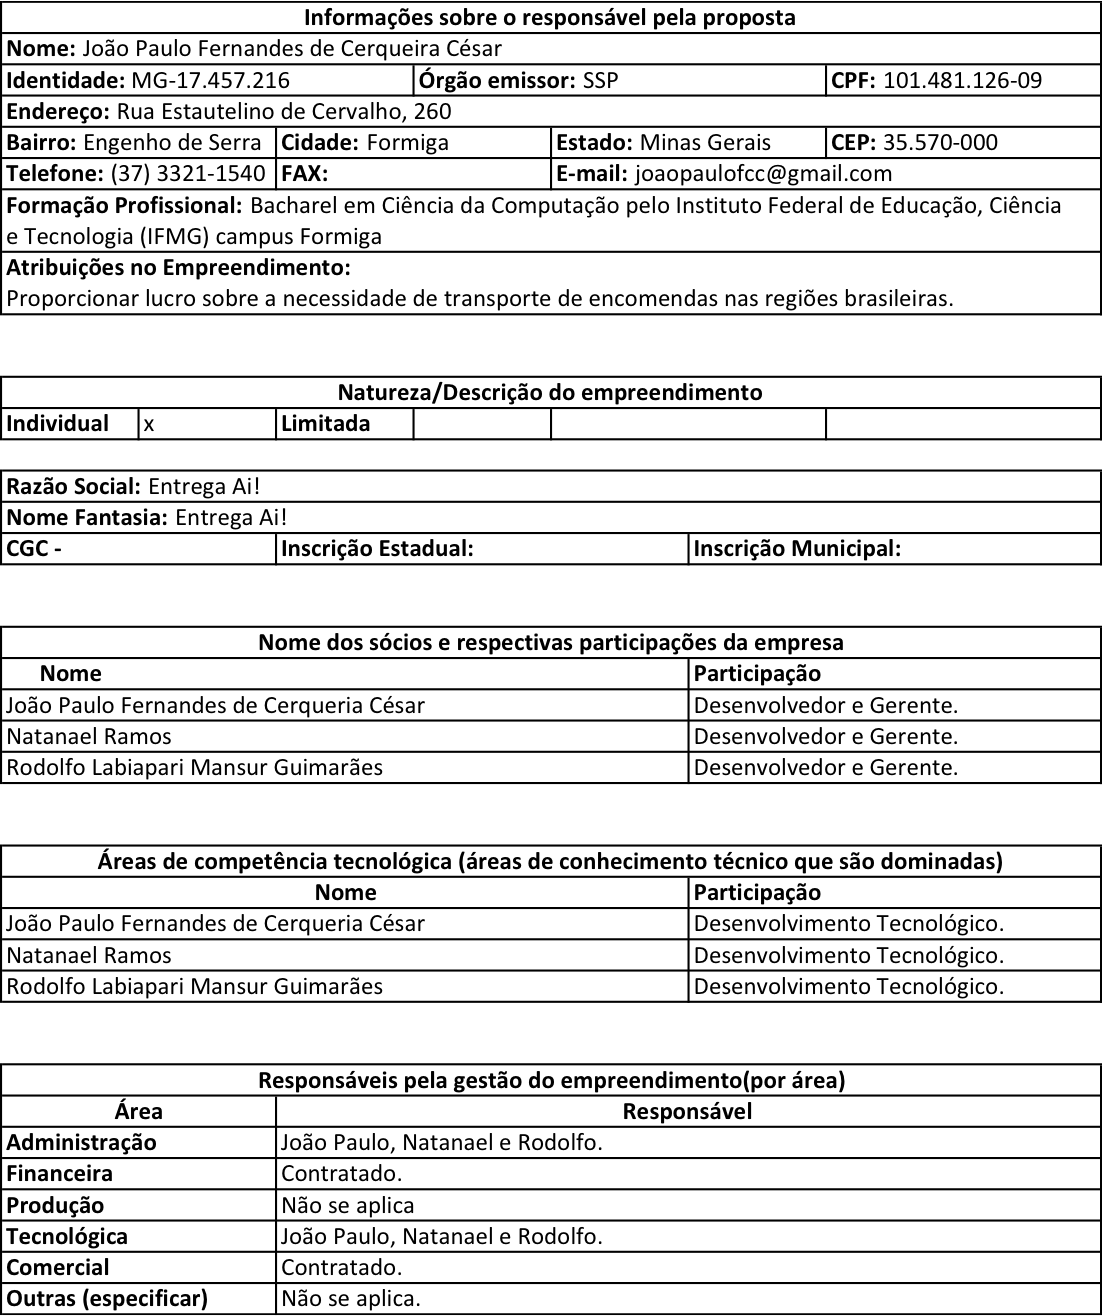
\includegraphics[width=1\linewidth]{img/1-1.png}
			\fonte{os autores}
		\end{table}
		\FloatBarrier
	
		A empresa, localizada no município de Formiga-MG, tem como objetivo a implantação do serviço on-line Entrega aí! onde realiza a intercomunicação facilitada do transportador e o embarcador. É uma ferramenta de prestação de serviço online onde realizar-se-á o fechamento de contrato entre interessados para que determinada carga seja enviada de um ponto até seu destino com segurança, rapidez e baixo custo.
		
		Na fase inicial da empresa não está prevista uma sede física, essa portanto funcioná de forma \textit{homeoffice} para cada colaborador. Inicialmente está previsto apenas a oferta do serviço online básico, ou seja, fornecer aos usuários um plataforma de qualidade. Entretanto, com a disseminação da tecnologia, popularização dos serviços prestados e boa avaliação da comunidade, será possível incrementar os serviços com meios mais fáceis de acesso, seguros e novidades na prestação de serviços.
        
        Abaixo, na \autoref{fig:logo}, é exibido a logomarca do Entrega Aí! criada pelos dirigentes.
        
        
		\begin{figure}[H]
			\centering
   			\caption{Logomarca da Empresa.}
			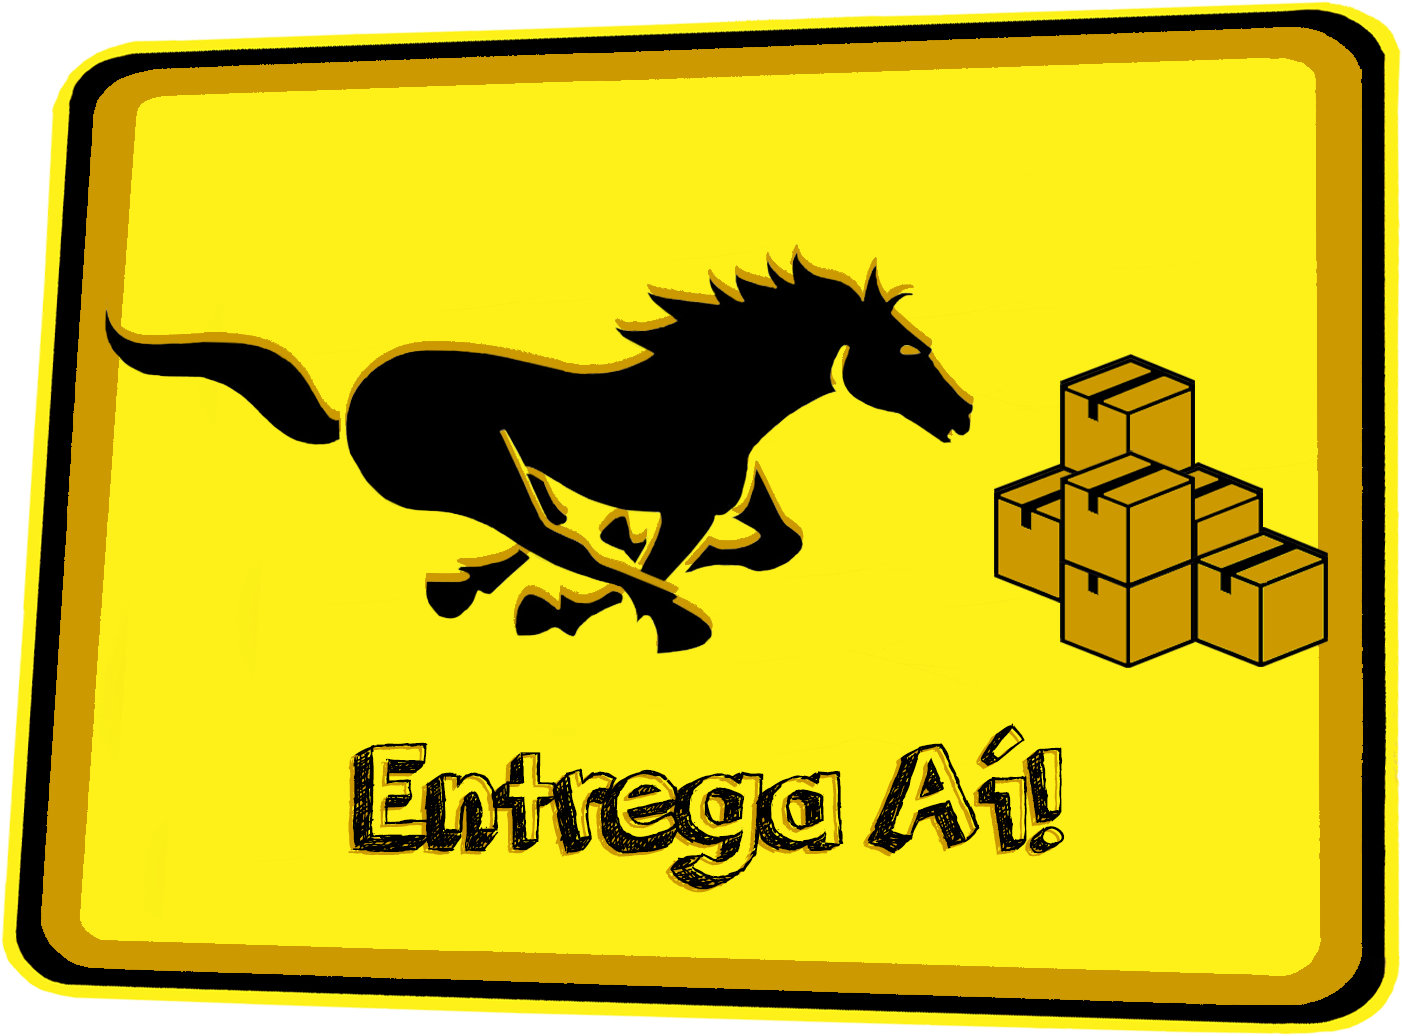
\includegraphics[width=0.8\linewidth]{img/logoEntregaAi.png}
			\fonte{os autores}
			\label{fig:logo}
		\end{figure}
		
	\section{Dados dos Dirigentes} \label{sec:dirigentes}
	
		Os dirigentes do negócio são também desenvolvedores do sistema, esses estão a par de como o sistema deve ser construído e utilizado, são eles:
		
			
		\begin{minipage}{0.6\textwidth}
			
			\textbf{João Paulo Fernandes de Cerqueira César}
			
			Bacharel em Ciência de Computação pelo IFMG \textit{campus} Formiga, 22 anos de idade, possui amplo interesse por tecnologia e inovação, coragem e determinação, além de gosto por situações novas e desafiadoras.
				
			
		\end{minipage}
		\begin{minipage}{0.4\textwidth}
			
			\begin{figure}[H]
				\centering
				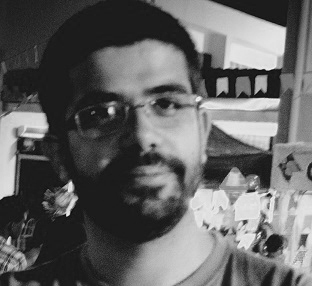
\includegraphics[width=0.65\textwidth]{img/jp2pb.jpg}
			\end{figure}
			
		\end{minipage}
		
		
		
		\begin{minipage}{0.6\textwidth}
			
			\textbf{Natanael Ramos}
				
			Bacharel em Ciência de Computação pelo IFMG \textit{campus} Formiga, 21 anos de idade, possui conhecimento em desenvolvimento de aplicações \textit{mobile} e amplo interesse em \textit{marketing}, além de ser um empreendedor nato.
				
			
		\end{minipage}
		\begin{minipage}{0.4\textwidth}
			
			\begin{figure}[H]
				\centering
				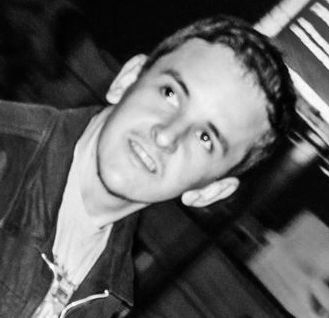
\includegraphics[width=0.65\textwidth]{img/noelpb.jpg}
			\end{figure}
			
		\end{minipage}
		
		
		
		\begin{minipage}{0.6\textwidth}
			
			\textbf{Rodolfo Labiapari Mansur Guimarães}
			
			Bacharel em Ciência de Computação pelo IFMG \textit{campus} Formiga, 21 anos de idade, possui conhecimento e experiência em desenvolvimento de sistemas web, além de paixão por inclusão digital.
				
			
		\end{minipage}
		\begin{minipage}{0.4\textwidth}
			
			\begin{figure}[H]
				\centering
				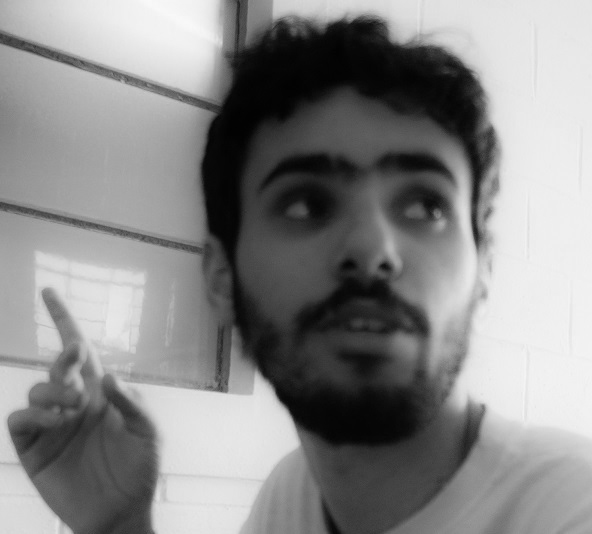
\includegraphics[width=0.65\textwidth]{img/dolfpb.jpg}
			\end{figure}
			
		\end{minipage}
				
		%\pagebreak
		
		No início, serão contratados auxiliares para gerenciamento das partes financeiras e contratuais da empresa além de um vendedor que fará representações buscando novos usuários e contratos/convênios, além da contratação de alguma agência de publicidade e propaganda para a disseminação divulgação do serviço de forma mais rápida.
	
	\section{Definição do Negócio}
		A abertura do negócio de entregas de mercadorias possui o objetivo de gerar lucros sobre a oportunidades existentes na região onde o serviço a ser prestado garante suprir a necessidade de possíveis usuários com problema de locomoção em suas mercadorias. O Plano de negócio aqui descrito é uma via de informações da empresa para o indivíduo requerido\footnote{\textit{Stakeholders}, Empréstimos, etc.}.
		
		A ideia geral do serviço pode ser entendida da seguinte maneira: 
		
		Embarcadores possuem encomendas que desejam enviar para outras localidades, diversos Transportadores, com diversos meios de transporte desejam realizar o frete de encomendas. Partindo então dessa premissa, Transportadores realizam um cadastro no site concordando com os termos e em seguida preenchem seu perfil, ou seja, quais meios de transporte possui à disposição dos Embarcadores, categorias de encomendas que possui interesse ou experiência de transporte deseja enviar. Os Embarcadores por sua vez, realizam o cadastro de forma semelhante ao dos Transportadores, e preenchem um perfil com as informações relativas a esse tipo de usuário. Após o cadastro, Embarcadores passam a ter acesso à plataforma, e assim, podem cadastrar encomendas que necessitam ser transportadas. De acordo com as características das encomendas, essas são exibidas aos Transportadores de maior interesse, que então determinam qual o preço que ele cobrará pelo frete, por último, o Embarcador que cadastrou a encomenda analisa qual o Transportador oferece o melhor serviço, e então o contrata. O serviço cuida de oferecer as melhores sugestões de usuários para seus propósitos (Embarcador para Transportadores e Transportador para Embarcador).

	\section{Fontes de Receita}
	
		Os custos iniciais da empresa serão fomentados pelos próprios dirigentes da empresa, devido ao fato de que o empreendimento não necessita de um alto investimento inicial. As metas para o primeiro mês da empresa preveem o pagamento das despesas iniciais e mensais, além disso, com o amadurecimento da empresa ao longo dos anos de serviço, será possível reinvestir na empresa, para assim melhorar os serviços providos. Portanto, nenhum empréstimo será necessário para a abertura da empresa.

	\section{Cenário Futuro para o Mercado}
	
		O fato da locomoção ser um problema em territórios extensos como o território brasileiro, condições de rodovias precárias e funcionamento inconsistente dos Correios, contribuem para o sucesso nacional deste sistema, que terá grande oportunidade de crescimento pela necessidade regional e consequentemente nacional.
		
		Após um período de consolidação da qualidade dos seus serviços a nível regional, a empresa, deverá almejar novos horizontes, ou seja, passará a atender usuários em todo o território nacional. Será necessário um processo intendo de publicidade fora da área regional da empresa, porém isso não caracteriza um problema, pois, para atingir essa fase a empresa deverá possuir capital social e financeiro a ser investido, admitindo sempre riscos calculados.

	\section{Visão}
	
		\begin{itemize}
			
			\item Abrangência geográfica , social e diversificada em relação aos tipos de produtos;
			
			\item Buscar ser referência em um modelo de entregas de qualidade.
			
		\end{itemize}

	\section{Missão}
	
		\begin{itemize}
			
			\item Trazer conforto ao Embarcador e produtividade a
			quem oferta os serviços de frete (Transportador)
			de forma fácil e prática;
			
			\item A empresa fornece um meio de comunicação
			direto entre o Embarcador e o Transportador.
			
		\end{itemize}

	\section{Estratégia}
	
	\subsection{Oportunidades}
	
		\begin{itemize}
			
			\item Disponibilidade de mão de obra técnica (manutenção do	\textit{software});
			
			\item Baixa concorrência na região com mesmo nível de serviços disponíveis;
			
			\item Popularização da internet e ferramentas computacionais;
			
			\item Popularização de ferramentas (web, mapas) para desenvolvimento;
			
			\item Crescimento do \textit{e-commerce};
			
			\item Frequente paralisações dos Correios.
			
		\end{itemize}
		
	\subsection{Ameaças}
	
		\begin{itemize}
			
			\item Restrições de horário dos Transportadores;
			
			\item Confiabilidade no serviço;
			
			\item Serviço sujeito à ineficiência devido a paralisação e qualidade das vias de transporte;
			
			\item Falta de compromisso e responsabilidade de Embarcadores e o Transportador;
			
			\item Dependência do funcionamento de serviços de camada inferior (internet).
			
		\end{itemize}
	
	\subsection{Forças}
		\begin{itemize}
			\item Praticidade de Uso;
			\item Interoperabilidade (compatibilidade com sites de compra);
			\item Privacidade;
			\item Histórico de Serviços (\textit{logs}, preços comparados, etc.);
			\item Categorização de serviços;
			\item Espaço para propaganda de serviços relacionados (Google AdWords, etc.);
			\item Diversificação dos Transportes;
			\item Otimização de roteamento (Caminho mais curto, rápido ou barato);
			\item Rastreamento (ativo ou passivo).
		\end{itemize}
		
		
	\subsection{Fraquezas}
		\begin{itemize}
			\item Comunicação (inclusão digital);
			\item Lucro da empresa por prover serviço pequeno;
			\item Disseminação (Disponibilidade de provedores de serviços, procura de clientes (Embarcadores/Transportadores));
		\end{itemize}
		
	
	\section{Infraestrutura}
		
		O empreendimento não necessita de nenhuma estrutura física para fornecer os serviços devido ao fato de ser \textit{home-office}. A única infraestrutura necessária será a locação de servidores para hospedagem do site e disponibilização dos serviços suprindo a quantidade de acesso necessária a visão de mercado atual da empresa.
	
	\section{Cronograma de Atividades}
	
	% Table generated by Excel2LaTeX from sheet '3-7'
	\begin{table}[H]
		\centering
		\caption{Cronograma de atividades}
		\begin{tabularx}{\linewidth}{|*4{>{\centering\arraybackslash}X|}}
			\toprule
			\textbf{Desenvolvimento do Serviço} & \textbf{Implantação do Serviço de Avaliação de usuário.} & \textbf{Implantação do Serviço de Recomendação de Pacotes.} & \textbf{Implantação do Serviço de Otimização de Rotas.} \\
			\midrule
			\textit{\textbf{Mês 1}} & \textbf{X} & \textbf{} & \textbf{} \\ [1.2ex] \hline
			\textit{\textbf{Mês 2}} & \textbf{X} & \textbf{} & \textbf{} \\ [1.2ex] \hline
			\textit{\textbf{Mês 3}} & \textbf{X} & \textbf{} & \textbf{} \\ [1.2ex] \hline
			\textit{\textbf{Mês 4}} & \textbf{X} & \textbf{X} & \textbf{} \\ [1.2ex] \hline
			\textit{\textbf{Mês 5}} & \textbf{} & \textbf{X} & \textbf{} \\ [1.2ex] \hline
			\textit{\textbf{Mês 6}} & \textbf{} & \textbf{X} & \textbf{X} \\ [1.2ex] \hline
			\textit{\textbf{Mês 7}} & \textbf{} & \textbf{X} & \textbf{X} \\ [1.2ex] \hline
			\textit{\textbf{Mês 8}} & \textbf{} & \textbf{X} & \textbf{X} \\ [1.2ex] \hline
			\textit{\textbf{Mês 9}} & \textbf{} & \textbf{} & \textbf{X} \\ [1.2ex] \hline
			\textit{\textbf{Mês 10}} & \textbf{} & \textbf{} & \textbf{X} \\ [1.2ex] \hline
			\textit{\textbf{Mês 11}} & \textbf{} & \textbf{} & \textbf{X} \\ [1.2ex] \hline
			\textit{\textbf{Mês 12}} & \textbf{} & \textbf{} & \textbf{X} \\ [1.2ex]
			\bottomrule
		\end{tabularx}%
		\label{tab:addlabel}%
	\end{table}%
    
    
    \chapter{A Proposta de Valor}
	\label{cap:APropostadeValor}
	
	\section{Quadro resumo dos serviços} \label{sec:servicos}
		
        Os preços adotados para os serviços ofertados variam de acordo com a capacidade de cada meio de transporte cadastrado pelo Transportador, e são cobrados mensalmente, como pode ser visto na \autoref{tab:precos}
        
    \begin{table}[H]
		\centering
		\caption{Tabela de preços dos serviços por capacidade.}
          \begin{tabularx}{\linewidth}{|X|c|c|}
          	  \toprule
			  \multicolumn{3}{c}{\cellcolor{gray!50}\textbf{Tabela de Preços por Serviço}} \\
			  \midrule
              \textbf{Veículo}             & \textbf{Preço} & \textbf{Acréscimo}                 \\
              \midrule
              \textit{Carretas}            & $R\$\ 80,00 $ & $+\ R\$\ 20,00 $ por carreta adicional \\ 
              \textit{Caminhões}           & $R\$\ 50,00 $ & ~                        \\
              \textit{Misto (Utilitários)} & $R\$\ 30,00 $ & ~                        \\
              \textit{Motos}               & $R\$\ 10,00 $ & ~                        \\
              \textit{Outros}              & $R\$\ 10,00 $ & ~                        \\
              \bottomrule
          \end{tabularx}
         
		\label{tab:precos}
	\end{table}
	%\FloatBarrier
	
	\section{Caracterização dos serviços}

		O Embarcador se cadastra gratuitamente no nosso serviço online e cadastra um pacote que ele deseja enviar para determinado destino.
		
		O Transportador se cadastra e cadastra pelo menos 1 (um) veículo. Cada veículo possui uma mensalidade de acordo com a tabela citada na Seção \ref{sec:servicos}.
		
		Após os cadastramentos, cada usuário poderá procurar por serviços ou mesmo ser sugeridos serviços por meio do sistema automático. Assim, cada transportador fará sua oferta de frete e o usuário escolhe a que mais lhe interessar.
	
	\section{Diferenciais dos serviços}
    
		\begin{itemize}
        
        	\item Um serviço de rota ótima (mínima, menos pedágios, melhores estradas) será oferecido ao Transportador para que ele obtenha um lucro máximo.
        
			\item Será possível que o embarcador escolha entre várias propostas de frete a melhor que satisfizer suas necessidades e requisições;
			
			\item O transportador poderá usufruir de um serviço onde exibirá outras encomendas que pertencem aquele trajeto que ele percorrerá aumentando seu lucro sobre pacotes transportados.
            
		\end{itemize}
	
	\section{Alianças estratégicas}
    
		O serviço Entrega Aí! usará serviços terceirizados para realizar convênios e propagandas para divulgação e parceria. Por exemplo, pode-se usar de contratos com vários postos de combustíveis, mecânicos, borracheiros, restaurantes, hotéis para que estes forneçam serviços especiais para usuários do Entrega Aí! além destes serem um meio de divulgação do sistema de entregas.
		
		Tais sociedades também podem realizar propaganda nos serviços online do Entrega Aí com a visão de aumentar a venda de seus serviços ou produtos.
	
	
	\chapter{O Mercado}
\label{cap:OMercado}
	
	\section{Sumário do Mercado}
	
	% Table generated by Excel2LaTeX from sheet '4-1'
	\begin{table}[htbp]
		\centering
		\small 
		\caption{Mercado Potencial Visado.}
		\begin{tabular}{rrrrrrr}
			\toprule
			\multicolumn{1}{c}{\multirow{2}[4]{*}{\textbf{}}} & \multicolumn{2}{c}{\textbf{Estimativa Mês 1}} & \multicolumn{2}{c}{\textbf{Estimativa Mês 2}} & \multicolumn{2}{c}{\textbf{Estimativa Mês 3}} \\
			\midrule
			\multicolumn{1}{c}{} & \multicolumn{1}{c}{\textbf{Total}} & \multicolumn{1}{c}{\textbf{Visado (\%)}} & \multicolumn{1}{c}{\textbf{Total}} & \multicolumn{1}{c}{\textbf{Visado (\%)}} & \multicolumn{1}{c}{\textbf{Total}} & \multicolumn{1}{c}{\textbf{Visado (\%)}} \\
			\textbf{Embarcadores} & 9     & 37.5  & 22    & 22.91 & 57    & 22.26 \\
			\textbf{Transportadores} & 15    & 62.5  & 72    & 75    & 191   & 74.615 \\
			\textbf{Patrocinadores} & 0     & 0     & 2     & 2.09  & 8     & 3.125 \\
			\textbf{Total} & 24    & 100\% & 96    & 100\% & 256   & 100\% \\
			\bottomrule
		\end{tabular}%
		\label{tab:addlabel}%
	\end{table}%
	
	\section{Público-Alvo}
		\begin{itemize}
			\item Empresas distribuidoras e freteiros;
			
			\item Variados cenários:
			\begin{itemize}
				\item Cidades pequenas;
				
				\item Locais distantes geograficamente.
			\end{itemize}
			
			\item Donos de veículos variados.
		\end{itemize}
	
	%\section{Tendência de crescimento dos segmentos de mercado}
	
	
	%\section{Participação pretendida por segmento de mercado}
	
	
	\section{Concorrência}
            
            
            
            
		\begin{minipage}{0.48\textwidth}
			\textbf{FreteBras:} 
			
            \begin{itemize}
              \item Cadastro de Embarcadores e Transportadores;
              \item Contato direto entre os dois;
              \item Suporte a dispositivo móvel;
              \item Check-in dos motoristas;
              \item Chat;
              \item R\$ 70,00 por mês para anunciantes de carga.
            \end{itemize}
				
		\end{minipage}
		\begin{minipage}{0.48\textwidth}
			
			\begin{figure}[H]
				\centering
				
\includegraphics[width=0.65\textwidth]{img/fretebras.png}
			\end{figure}
			
		\end{minipage}
        \bigskip
            
            
            
            
		\begin{minipage}{0.48\textwidth}
			
			\textbf{Frete na Mão:}
				\begin{itemize}
					\item Cadastro de Embarcadores e Transportadores;
					\item Contato direto entre os dois;
					\item Divulgação de utilitários na estrada;
					\item Cotação de frete;
				\end{itemize}
                
		\end{minipage}
		\begin{minipage}{0.48\textwidth}
			
			\begin{figure}[H]
				\centering
				
\includegraphics[width=0.65\textwidth]{img/frete-na-mao.png}
			\end{figure}
			
		\end{minipage}
        \bigskip
                
                
            
		\begin{minipage}{0.48\textwidth}
			
			\textbf{Axado:}
				\begin{itemize}
					\item Cálculo de tabela de frete;
					\item Buscapé dos fretes;
					\item Trabalho exclusivo com transportadoras;
					\item Geração de relatórios;
					\item Campanha de frete grátis;
					\item Planos começam em R\$ 1000,00 por mês.
				\end{itemize}
		\end{minipage}
		\begin{minipage}{0.48\textwidth}
			
			\begin{figure}[H]
				\centering
				
\includegraphics[width=0.65\textwidth]{img/axado.png}
			\end{figure}
            
		\end{minipage}
        \bigskip
        
        
				
		\begin{minipage}{0.48\textwidth}
			
			\textbf{TEMFrete:}
				\begin{itemize}
					\item Cadastro de Embarcadores e Transportadores;
					\item Contato direto entre os dois;
					\item Variabilidade nos tipos de transporte:
					\begin{itemize}
						\item Aéreo;
						\item Marítimo;
						\item Fluvial;
						\item Ferroviário;
						\item Rodoviário.
					\end{itemize}
				\end{itemize}
		\end{minipage}
		\begin{minipage}{0.48\textwidth}
			
			\begin{figure}[H]
				\centering
				
\includegraphics[width=0.65\textwidth]{img/temfrete.png}
			\end{figure}
			
		\end{minipage}
				
                
	
	\section{Diferencial competitivo}
		\begin{itemize}
			\item Otimização de rotas com algoritmos da própria empresa.
			
			\item Aumento de lucro do entregador visando obter mais encomendas sobre determinado trajeto realizando sugestões de entregas que estiverem situadas no percurso especificado da viagem principal do transportador.
			
			\item Avaliações e comentários de Embarcadores e Transportadores criando reputações.
			
			\item Interoperabilidade com \textit{e-commerce} criando uma possível possibilidade de escolha de envio do pacote usando o serviço por nós oferecido.
		\end{itemize}
	
	%\section{Metas específicas de vendas}
	
	
	\chapter{A Estratégia de Marketing e Vendas}
\label{cap:marketing}
	
	\section{Política de preços}
		O serviço provê oportunidade de adicionar publicidade no site para auxiliar nos custos da empresa em troca de exibir serviços de terceiros.
		
		Apoio de futuros investimentos de patrocinadores do serviço.
		
		Serviços adicionais de cobrança como:
		\begin{itemize}
			\item Consulta a serviços de manutenção mais próximos;
			\item Serviços de otimização ilimitados;
			\item Contato direto com empresas transportadoras para oferta de emprego.
		\end{itemize}
	
	\section{Ações de marketing e vendas}
		Venda direta através de um vendedor ambulante para que traga mais pessoas e empresas para o serviço a fim de aumentar os usuários em uso.
		
		Convênio com empresas transportadoras para ofertas de mercadorias especiais ou priorizadas.
		
		E também, recursos online tal como publicidade de comunicação tal como \textit{YouTube}, \textit{Twitter}, \textit{Facebook} entre muitos outros.
	
	\section{Cronograma de atividades do marketing e vendas}
		Inicialmente será utilizado como meio de divulgação o vendedor no qual tentará realizar contratos com empresas e sociedades e também meios de comunicação baratos e que disseminam rapidamente além de propaganda na região implantada.
	
	
	\chapter{As Finanças}
\label{cap:financas}
	
	\section{Investimentos iniciais}
	
        \subsection{Despesas Pré-Operacionais}
	% Table generated by Excel2LaTeX from sheet '3-7'
	\begin{table}[htbp]
		\centering
		\caption{Custos Iniciais}
		
			\begin{tabularx}{\linewidth}{|X|c|c|}
				\toprule
				\multicolumn{3}{c}{\cellcolor{gray!50}\textbf{Custos Iniciais}} \\
				\midrule
				\textbf{Nome do Serviço} & \textbf{Quantidade} & \textbf{Preço R\$} \\
				\midrule
				\textit{Uniformes}					&	8	& 120,00 \\
				\textit{Materiais de Divulgação}	&	NA	& 400,00 \\
				\textit{Cadastro Empresa}			&	NA	& 400,00 \\
				\textit{Notebook Vendedor}			&	1	& 1.600,00 \\
				\textit{Registro Domínio - 5 Anos}	&	1	& 138,00 \\
                \midrule
				~ & \textbf{Total} & \textbf{2.258,00} \\
				\bottomrule
			\end{tabularx}
		
		\label{tab:previas}%
	\end{table}%
	
    
	\section{Origem dos recursos}
		Todos os investimentos iniciais serão providos dos próprios gerentes da empresa. O motivo de utilizar os próprios recursos para os investimentos de inicialização desta para evitar quaisquer tipos de empréstimos e consequentemente juros a pagar.
	
    
    
    
	\section{Receita e custos}
		
        \subsection{Custo Fixo}
		
		% Table generated by Excel2LaTeX from sheet '3-7'
		\begin{table}[htbp]
			\centering
			\caption{Custos Fixos}
			
			
			\begin{tabularx}{\linewidth}{|X|c|c|}
				\toprule
				\multicolumn{3}{c}{\cellcolor{gray!50}\textbf{Custos Fixos}} \\
				\midrule
				\textbf{Nome do Serviço} & \textbf{Quantidade} & \textbf{Preço R\$} \\
				\midrule
				\textit{Aluguel Servidor Dedicado}		&	1	& 800,00 \\
				\textit{Hospedagem Site - Pagamento Trienal}		&	1	& 10,00 \\
				\textit{Gasolina}						&	50 l& 200,00 \\
				\textit{Contador}						&	1	& 400,00 \\
				\textit{Vendedor}						&	1	& 800,00 \\
				\textit{Desenvolvedor}					&	3	& 3.000,00 \\
                \midrule
				\textbf{Total}									& ~ & \textbf{5.210,00} \\
				\bottomrule
			\end{tabularx}
			
			
			\label{tab:receitasfixas}%
		\end{table}%
        
        
        
        \subsection{Investimento Inicial}
        
		% Table generated by Excel2LaTeX from sheet '3-7'
		\begin{table}[htbp]
			\centering
			\caption{Investimento Inicial.}
			
			
				\begin{tabularx}{\linewidth}{|X|c|}
					\toprule
					\multicolumn{2}{c}{\cellcolor{gray!50}\textbf{Investimento Inicial}} \\
					\midrule
					\textbf{Descrição} & \textbf{Valor}  \\
					\midrule
					\textit{Despesas Pré-Operacionais}		&	2.258,00 \\
					\textit{Capital de Giro}	&	5.510,00 \\
					\midrule
					\textbf{Total}			& \textbf{7.468,00} \\
					\bottomrule
				\end{tabularx}
			
			
			\label{tab:investimentoInicial}%
		\end{table}%
        
        
        
        \subsection{Receitas e Comissão}
		
		% Table generated by Excel2LaTeX from sheet '3-7'
		\begin{table}[htbp]
			\centering
			\caption{Total Receitas.}
			
			
			\begin{tabularx}{\linewidth}{|X|c|c|c|}
				\toprule
				\multicolumn{4}{c}{\cellcolor{gray!50}\textbf{Total Receitas}} \\
				\midrule
				\textbf{Descrição} & \textbf{Mês 1} & \textbf{Mês 2} & \textbf{Mês 3} \\
				\midrule
				\textit{Receitas à vista}			&	6.000,00	& 6.500,00 & 7.000,00 \\
				\textit{Receitas operacionais (Soma das receitas)}	&	6.000,00	& 6.500,00 & 7.000,00 \\
				\textit{(-) Comissão de vendas (5\%)}	&	300,00	& 325,00 & 350,00 \\
				\bottomrule
			\end{tabularx}
			
			
			\label{tab:receitasEComissoes}%
		\end{table}%
		
        
        
        \subsection{Impostos e Contribuições}
		
		% Table generated by Excel2LaTeX from sheet '3-7'
		\begin{table}[htbp]
			\centering
			\caption{Impostos e Contribuições.}
			
			
				\begin{tabularx}{\linewidth}{|X|c|c|c|c|}
					\toprule
					\multicolumn{5}{c}{\cellcolor{gray!50}\textbf{Impostos Impostos e Con Contribuiçõeribuições.}} \\
					\midrule
					\textbf{Descrição} & \textbf{Alíquota} & \textbf{Mês 1} & \textbf{Mês 2} & \textbf{Mês 3} \\
					\midrule
					\textit{Simples Nacional (Super Simples)}&	0\%		& 44,40 	& 44,40 & 44,40 \\
					\midrule
					\textbf{Total}			&	~	& \textbf{44,40} 	& \textbf{44,40} & \textbf{44,40} \\
					\bottomrule
				\end{tabularx}
			
			
			\label{tab:inpostosEContribuicoes}%
		\end{table}%
		
        
        
        \subsection{Total de deduções}
        
        
		% Table generated by Excel2LaTeX from sheet '3-7'
		\begin{table}[htbp]
			\centering
			\caption{Total de deduções.}
			
			
				\begin{tabularx}{\linewidth}{|X|c|c|c|}
					\toprule
					\multicolumn{4}{c}{\cellcolor{gray!50}\textbf{Total de deduções.}} \\
					\midrule
					\textbf{Descrição} & \textbf{Mês 1} & \textbf{Mês 2} & \textbf{Mês 3}	\\
					\midrule
					\textit{Comissão de vendas (5\%)}	&	300,00	& 325,00 	& 350,00 	\\
					\textit{Impostos e Contribuições}	& 	44,40 	& 44,40 	& 44,40 	\\
					\midrule
					\textbf{Total}						&	\textbf{344,40} 	& 	\textbf{369,40} 	& \textbf{394,40} 	\\
					\bottomrule
				\end{tabularx}
			
			
			\label{tab:totalDeducoes}%
		\end{table}%
		
        
        
        \subsection{Demonstrações de Resultados}
        
		% Table generated by Excel2LaTeX from sheet '3-7'
		\begin{table}[H]
			\centering
			\caption{Demonstrações de Resultados.}
			
				\begin{tabularx}{\linewidth}{|X|c|c|c|}
					\toprule
					\multicolumn{4}{c}{\cellcolor{gray!50}\textbf{Demonstrações de Resultados.}} \\
					\midrule
					\textbf{Descrição} & \textbf{Mês 1} & \textbf{Mês 2} & \textbf{Mês 3} \\
					\midrule
					\textit{Receita Bruta de Vendas}						&	6.000,00		& 6.500,00		 & 7.000,00 \\
					\textit{(-) Deduções (Impostos, comissões, abatimentos}	& 5.554,40 			& 5.579,40 		& 5.604,40 \\
                    \midrule
					\textbf{Lucro líquido}									& \textbf{445,60} 	& \textbf{92,60} & \textbf{1.395,60} \\
					\bottomrule
				\end{tabularx}
			
			
			\label{tab:Demonstracoes}%
		\end{table}%
        
        
        \subsection{Fluxo de Caixa Mensal}
        
		% Table generated by Excel2LaTeX from sheet '3-7'
		\begin{table}[H]
			\centering
			\caption{Fluxo de Caixa Mensal.}
			
			
				\begin{tabularx}{\linewidth}{|c|X|c|c|c|c|}
					\toprule
					\multicolumn{6}{c}{\cellcolor{gray!50}\textbf{Fluxo de Caixa Mensal.}} \\
					\midrule
					\textbf{Item} & \textbf{Descrição} 						& \textbf{(*)} & \textbf{Mês 1} & \textbf{Mês 2} & \textbf{Mês 3} \\
					\midrule
					\textbf{1}   & \textit{Investimento Inicial}			& 7.468,00	& ~  		& ~ 		& ~ \\
					\textbf{2.1} & \textit{(+) Total de Entrada} 			&	~		&	0,00 	& 445,60 	& 1366,20  \\
					\textbf{2.2} & \textit{(+) Patrocinadores}				&	~		&	6.000	&	6,500,00 & 7.000,00  \\
                    \textbf{2.2} & \textit{(+) Receita de Vendas}			&	~		&	315,00	& 505,00	& 605,00	\\
                    \textbf{2} 	 & \textbf{Saldo de Caixa Inicial}			&	~		&	5.685,00& 5995,00	& 6.395,00	\\
                    \textbf{3.1} & \textit{(-) Deduções (Impostos, Comissões)} & ~  	& - 5.554,40& - 5579,40	& - 5.604,40 \\	
                    \textbf{3.2} & \textit{(-) Despesas Operacionais (fixas)} &	~		& - 344,40	& - 369,40	& - 394,40	\\
                    \textbf{3} & \textbf{Total de Saídas} 					&	~		&	-5.210,00&- 5.210,00& - 5,210,00\\	
                    \midrule
                    ~			 &   \textbf{Saldo Acumulado de Caixa} 				&	~		& \textbf{445,60}	& \textbf{1366,20}	& \textbf{2.761,80}	\\
					\bottomrule
				\end{tabularx}
			
			
			\label{tab:FluxoCaixa}
        \end{table}
	
	
	%% ---
% Finaliza a parte no bookmark do PDF
% para que se inicie o bookmark na raiz
% e adiciona espaço de parte no Sumário
% ---
\phantompart

% ---
% Conclusão
% ---
\chapter*[Conclusão]{Conclusão}
	
	
	% ----------------------------------------------------------
	% ELEMENTOS PÓS-TEXTUAIS
	% ----------------------------------------------------------
	\postextual
	
	% ----------------------------------------------------------
	% Referências bibliográficas
	% ----------------------------------------------------------
	\bibliography{bibliografia}
	
	
\end{document}
